%
% lf.tex
%
% (c) 2026 Prof Dr Andreas Müller
%
\begin{figure}
\centering
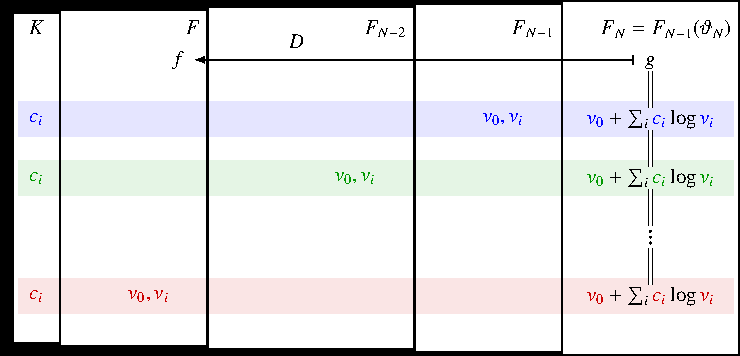
\includegraphics{chapters/070-intalg/images/lf.pdf}
\caption{Allgemeiner Fall des Prinzips von Liouville.
Die Stammfunktion $g\in F_N$ lässt sich in Liouville-Form
bezüglich $F_{N-1}\subset F_N$ mit den blauen Elementen
${\color{blue}c_i}\in K$ und
${\color{blue}v_0}, {\color{blue}v_i}\in F_{N-1}$
schreiben.
Sie muss schrittweise durch neue Elemente in anderen Farben 
in Liouville-Form bezüglich Erweiterungen $F_{k-1}\subset F_k$
umgeschrieben werden, bis die endgültige Liouville-Form mit
roten Elementen ${\color{darkred}c_i}\in K$ und
${\color{darkred}v_0}, {\color{darkred}v_i}\in F$ entsteht.
Dies beweist das Prinzip von Liouville.
\label{buch:intalg:liouville:fig:lf}}
\end{figure}
